In this study, we employed several machine learning techniques to model and analyze the synthetic terrain data generated by the Franke Function. The primary focus was on implementing and comparing the performance of Ordinary Least Squares (OLS), Ridge regression, and Lasso regression. To ensure the robustness and reliability of our results, we utilized data preprocessing techniques and validation methods, including train-test splitting, feature scaling, cross-validation, and bootstrapping.

\subsection{Data Generation and Preprocessing}

The synthetic dataset was generated using the Franke Function equation \ref{eq:frankefunction} over a grid of $(x, y)$ values from the uniform distribution. To simulate real-world data imperfections, normally distributed noise was added to the output $f(x, y)$. We used the seed "2024" to create consistent data. The resulting dataset was then prepared for regression analysis. The real terrain data was taken from the file \texttt{SRTM\_data\_Norway\_1.tif} from the course datafiles \cite{CompPhysics2023}.

\begin{equation}
\begin{split}    
    f(x, y) = & \ \frac{3}{4} e^{-\frac{(9x-2)^2}{4} - \frac{(9y-2)^2}{4}} + \frac{3}{4} e^{-\frac{(9x+1)^2}{49} - \frac{(9y+1)}{10}} \\
    & + \frac{1}{2} e^{-\frac{(9x-7)^2}{4} - \frac{(9y-3)^2}{4}} - \frac{1}{5} e^{-(9x-4)^2 - (9y-7)^2}
   \label{eq:frankefunction}
\end{split}
\end{equation}

\subsubsection{Train-Test Split}

To evaluate the predictive performance of the models, the dataset was split into training and testing sets using the \texttt{train\_test\_split} function from the \texttt{scikit-learn} library \cite{scikit-learn}. The data was partitioned such that 80\% was used for training and 20\% for testing. This split ensures that the models are trained on a substantial portion of the data while reserving a separate set for unbiased evaluation.

\subsubsection{Feature Scaling}

Feature scaling is crucial for algorithms that are sensitive to the magnitude of the features, especially when regularization is involved. Without scaling, the features with larger values will be penalized more than those with small values. We scaled the variables using the \texttt{StandardScaler} from \texttt{scikit-learn}. Standardization transforms the data to have zero mean and unit variance, computed as:

\begin{equation}
    z = \frac{x - \mu}{\sigma}
\end{equation}

where $x$ is the original feature value, $\mu$ is the mean, and $\sigma$ is the standard deviation of the feature values in the training set. By centering the data, we reduce the multicollinearity of the columns with higher power in the design matrix. This makes our model more numerically stable. It can also reduce the risk of our design-matrix becoming nearly-singular, which makes computation easier.\cite{polyreg_budescu}

A downside with using the standard scaler is that it doesn´t provide a minimum and a maximum value for our data set. \cite{Hjorth-Jensen_MachineLearning_2023} However, it is both really easy to understand and easy to implement, which we weighed more.

The scaler was fit on the training data and then applied to both training and test sets to prevent data leakage between the two. When using cross-validation later on, we should ideally have scaled the data in each fold \ref{algo:kfold} for the same reason, but for simplicity and consistency of our code, we decided against it. 

 Although real data often benefits more from scaling than "perfect" data generated from a uniform distribution with mean zero, we scaled both the synthetic data and the terrain data to be consistent throughout the project. When trying to recreate our real data later on, we had to do an inverse scaling to get the correct values. 


\subsection{Regression Techniques}

The following regression techniques were implemented:

\subsubsection{Ordinary Least Squares (OLS)}

OLS served as the baseline model without regularization, optimized by minimizing the residual sum of squares in equation \ref{eq:betaOLS}. The model was fitted using the closed-form solution provided by the normal equation.

\begin{equation}
    \boldsymbol{\beta}_{\text{OLS}} = (\mathbf{X}^T \mathbf{X})^{-1} \mathbf{X}^T \mathbf{y}
    \label{eq:betaOLS}
\end{equation}

\subsubsection{Ridge Regression}

Ridge regression introduces an $L2$ penalty term to shrink the coefficients, controlled by a regularization parameter $\lambda$. The objective function to minimize equation \ref{eq:Ridgeminimize}.

\begin{equation}
       \text{Ridge:} \quad \min_{\boldsymbol{\beta}} \left\{ \sum_{i=1}^{n} (y_i - \hat{y}_i)^2 + \lambda \sum_{j=1}^{p} \beta_j^2 \right\}
    \label{eq:Ridgeminimize}
\end{equation}

where $\lambda$ is the regularization parameter, and $p$ is the number of predictors. The solution for the Ridge regression coefficients is as described in equation \ref{eq:betaRidge}:

\begin{equation}
    \boldsymbol{\beta}_{\text{Ridge}} = (\mathbf{X}^T \mathbf{X} + \lambda \mathbf{I})^{-1} \mathbf{X}^T \mathbf{y}
    \label{eq:betaRidge}
\end{equation}

We used grid search combined with 20-fold cross-validation to find the optimal value of $\lambda$. The search spanned a range of $\lambda$ values on a logarithmic scale to capture both small and large regularization effects.

\subsubsection{Lasso Regression}
\begin{figure}[h]
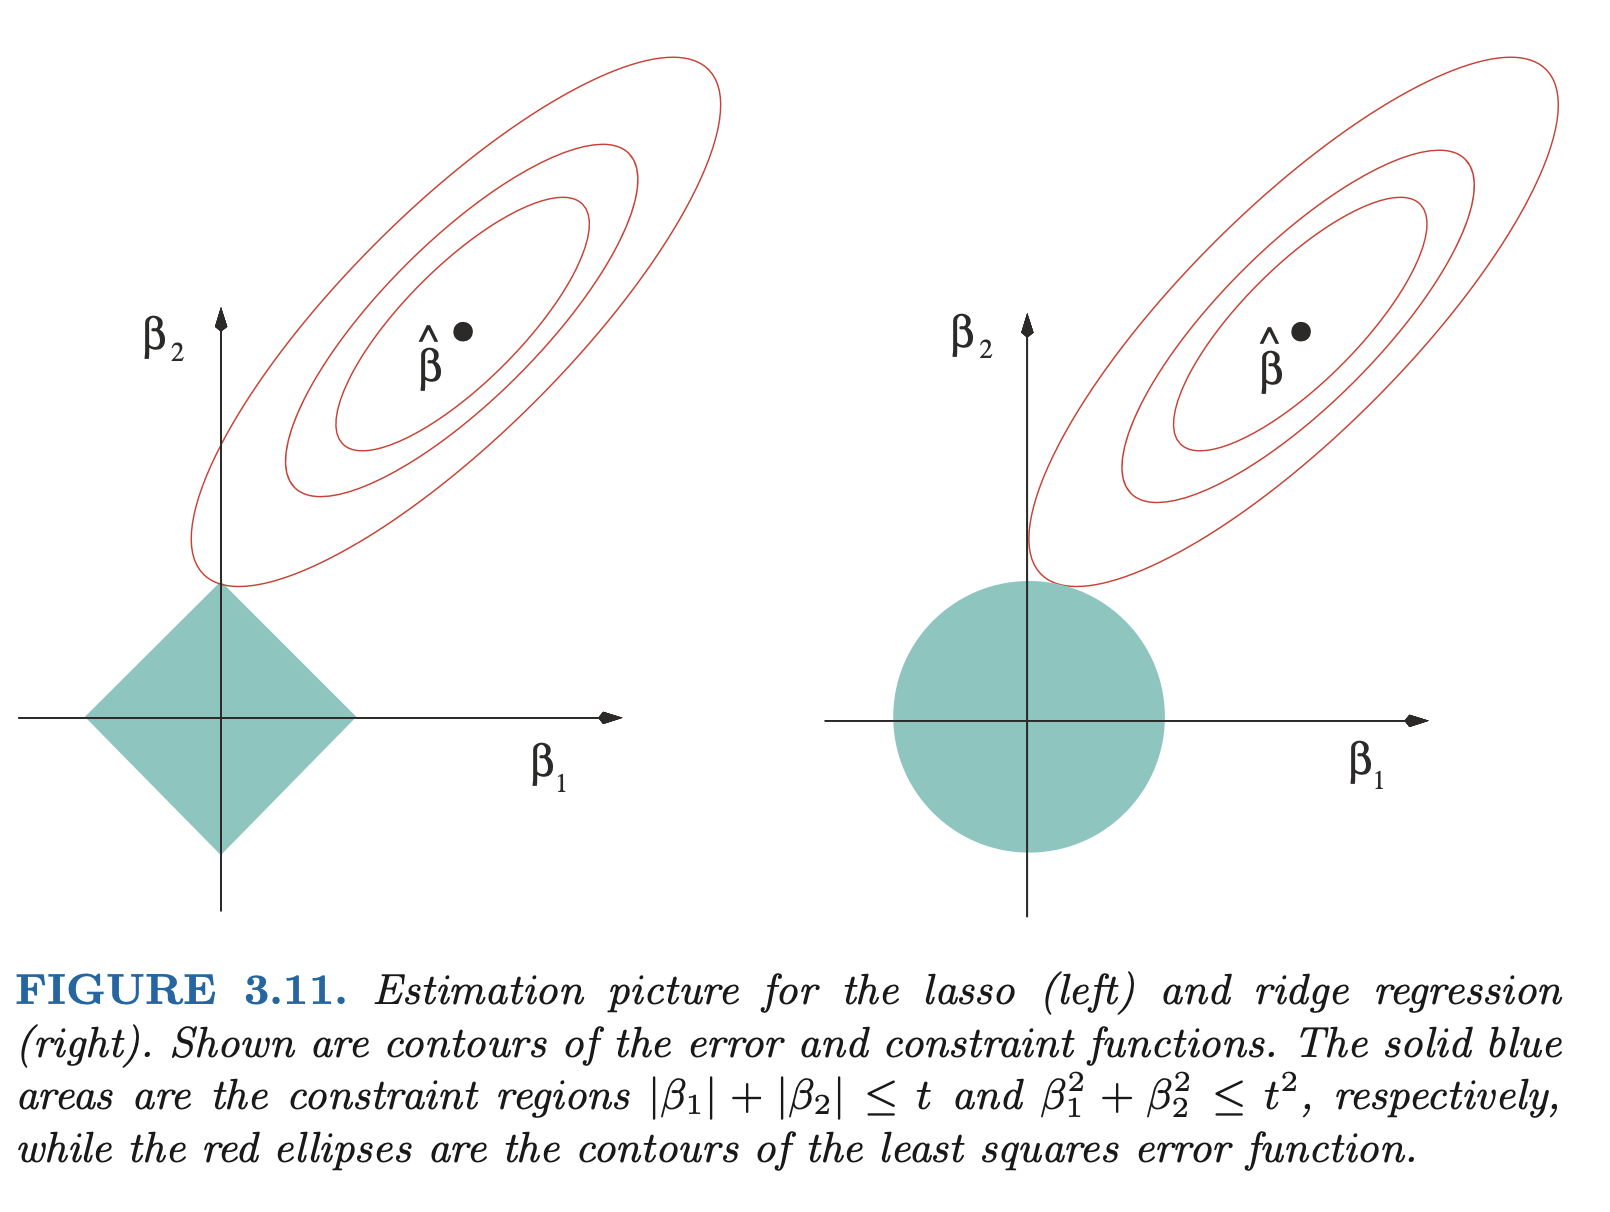
\includegraphics[width=8cm]{method_ridge_vs_lasso.png}
\caption{We have here borrowed figure 3.11 from ESL to illustrate the difference between how the L1 and L2 norm shrinks the parameters. \cite{ESL}}
\label{fig:L1vsL2}
\end{figure}

Lasso regression incorporates an $L1$ penalty to promote sparsity in the coefficients, controlled by the regularization parameter $\lambda$. The objective was to miminize beta in equation \ref{eq:Lassominimize}. 

\begin{equation}
    \text{Lasso:} \quad \min_{\boldsymbol{\beta}} \left\{ \sum_{i=1}^{n} (y_i - \hat{y}_i)^2 + \lambda \sum_{j=1}^{p} |\beta_j| \right\}
    \label{eq:Lassominimize}
\end{equation}

From figure \ref{fig:L1vsL2} we see that the constraint region imposed by $L1$ (left) makes it more likely that the optimal $\beta$ (where the OLS estimate $\hat{\beta}$ meets the constraint region) is zero, than for Ridge regression (right). 

Similar to Ridge regression, we used grid search and 10-fold cross-validation to select the optimal $\lambda$. The $L1$ penalty tends to set some coefficients exactly to zero, effectively performing feature selection.

\subsubsection{Expectation and variance in linear regression}
In the context of ordinary least squares (OLS), the vector of observations $( \mathbf{y} )$ is modeled as:
$$\mathbf{y} = \mathbf{X} \boldsymbol{\beta} + \boldsymbol{\epsilon}$$
For each element $( y_i )$ in the vector $( \mathbf{y} )$, we have:
$$y_i = \sum_j x_{ij} \beta_j + \epsilon_i$$
where $( x_{ij} )$ is the element in the $( i )-th$ row and $( j )-th$ column of the matrix $( \mathbf{X} )$, and $( \epsilon_i )$ is the corresponding error for the $( i )-th$ observation.
We then take the expectation of $y_i$.
$$\mathbb{E}(y_i) = \mathbb{E}\left( \sum_j x_{ij} \beta_j + \epsilon_i \right)$$
By the linearity of expectation, we have that:
$$\mathbb{E}(y_i) = \sum_j x_{ij} \beta_j + \mathbb{E}(\epsilon_i)$$
Since $( \epsilon_i )$ is normally distributed with mean 0, we have:
$$\mathbb{E}(\epsilon_i) = 0$$
$$\mathbb{E}(y_i) = \sum_j x_{ij} \beta_j$$
In matrix form, this can be written as:
$$\mathbb{E}(y_i) = \mathbf{X}_{i,*} \boldsymbol{\beta}$$
where $( \mathbf{X}_{i,*} )$ is the $( i )-th$ row of the design matrix $( \mathbf{X} )$
Thus the expectation value of $( y_i )$ is:
$$\mathbb{E}(y_i) = \sum_j x_{ij} \beta_j = \mathbf{X}_{i,*} \boldsymbol{\beta}$$

We then find the variance
$$\text{Var}(y_i) = \text{Var}\left(\sum_j x_{ij} \beta_j + \epsilon_i\right)$$

Since the deterministic part $( \sum_j x_{ij} \beta_j )$ is constant with respect to the random error $( \epsilon_i )$, its variance is 0. Thus, we have:

$$\text{Var}(y_i) = \text{Var}(\epsilon_i)$$

From the assumptions, we know that $(\epsilon_i \sim N(0, \sigma^2))$, so:

$$\text{Var}(\epsilon_i) = \sigma^2$$

Thus, we can then conclude that:

$$\text{Var}(y_i) = \sigma^2$$

The OLS estimator for the regression coefficients $( \hat{\beta} )$ is given by the well-known formula:

$$\hat{\beta} = (\mathbf{X}^\top \mathbf{X})^{-1} \mathbf{X}^\top \mathbf{y}$$


By substituting $( \mathbf{y} = \mathbf{X} \beta + \boldsymbol{\epsilon} )$ into the expression for $( \hat{\beta} )$ we get:

$$\hat{\beta} = (\mathbf{X}^\top \mathbf{X})^{-1} \mathbf{X}^\top (\mathbf{X} \beta + \boldsymbol{\epsilon})$$

Using the distributive property of matrix multiplication:

$$\hat{\beta} = (\mathbf{X}^\top \mathbf{X})^{-1} \mathbf{X}^\top \mathbf{X} \beta + (\mathbf{X}^\top \mathbf{X})^{-1} \mathbf{X}^\top \boldsymbol{\epsilon}$$

The first term simplifies because $( (\mathbf{X}^\top \mathbf{X})^{-1} \mathbf{X}^\top \mathbf{X} = \mathbf{I} )$:

$$\hat{\beta} = \beta + (\mathbf{X}^\top \mathbf{X})^{-1} \mathbf{X}^\top \boldsymbol{\epsilon}$$

Now, we take the expectation of both sides:

$$\mathbb{E}[\hat{\beta}] = \mathbb{E}[\beta + (\mathbf{X}^\top \mathbf{X})^{-1} \mathbf{X}^\top \boldsymbol{\epsilon}]$$

Since $( \beta )$ is a constant and the expectation operator is linear:

$$\mathbb{E}[\hat{\beta}] = \beta + \mathbb{E}[(\mathbf{X}^\top \mathbf{X})^{-1} \mathbf{X}^\top \boldsymbol{\epsilon}]$$

The term $( (\mathbf{X}^\top \mathbf{X})^{-1} \mathbf{X}^\top \boldsymbol{\epsilon} )$ involves the error $( \boldsymbol{\epsilon} )$, and since $( \mathbb{E}[\boldsymbol{\epsilon}] = 0 )$, we have:

$$\mathbb{E}[(\mathbf{X}^\top \mathbf{X})^{-1} \mathbf{X}^\top \boldsymbol{\epsilon}] = 0$$

Which means that: 

$$\mathbb{E}[\hat{\beta}] = \beta$$

To find the variance of Beta, we use the expression for the OLS estimator:

$$\hat{\beta} = (\mathbf{X}^\top \mathbf{X})^{-1} \mathbf{X}^\top \mathbf{y}$$

Using the model $( \mathbf{y} = \mathbf{X} \beta + \boldsymbol{\epsilon} )$, we substitute this into the expression for $( \hat{\beta} )$:

$$\hat{\beta} = (\mathbf{X}^\top \mathbf{X})^{-1} \mathbf{X}^\top (\mathbf{X} \beta + \boldsymbol{\epsilon})$$

This simplifies to:
$$\hat{\beta} = \beta + (\mathbf{X}^\top \mathbf{X})^{-1} \mathbf{X}^\top \boldsymbol{\epsilon}$$

We now want to compute the variance of $( \hat{\beta} )$. The variance operator acts only on the random error term $( \boldsymbol{\epsilon} )$, since $( \beta )$ is deterministic.

Thus, the variance of $( \hat{\beta} )$ is:

$$\text{Var}(\hat{\beta}) = \text{Var}\left((\mathbf{X}^\top \mathbf{X})^{-1} \mathbf{X}^\top \boldsymbol{\epsilon}\right)$$

Using the fact that for a random vector $( \mathbf{A} \mathbf{Z} ),$ where $( \mathbf{Z} )$ is a random vector and $( \mathbf{A} )$ is a matrix, the variance is:

$$\text{Var}(\mathbf{A} \mathbf{Z}) = \mathbf{A} \, \text{Var}(\mathbf{Z}) \, \mathbf{A}^\top$$

Here, $( \mathbf{A} = (\mathbf{X}^\top \mathbf{X})^{-1} \mathbf{X}^\top )$ and $( \boldsymbol{\epsilon} \sim N(0, \sigma^2 \mathbf{I}))$. The variance of $( \boldsymbol{\epsilon} )$ is:

$$\text{Var}(\boldsymbol{\epsilon}) = \sigma^2 \mathbf{I}$$

Which means that the variance of $( \hat{\beta} )$ becomes:

$$\text{Var}(\hat{\beta}) = (\mathbf{X}^\top \mathbf{X})^{-1} \mathbf{X}^\top \, \sigma^2 \mathbf{I} \, \mathbf{X} \, (\mathbf{X}^\top \mathbf{X})^{-1}$$

This simplifies to:

$$\text{Var}(\hat{\beta}) = \sigma^2 (\mathbf{X}^\top \mathbf{X})^{-1}$$
\subsection{Model Training and Validation}

\subsubsection{Cross-Validation with K-Folds}

To assess the models' generalization capability and to avoid overfitting, we employed $K$-fold cross-validation with $K = 10$. In this method, the training data is partitioned into 10 subsets (folds). The model was trained on $k-1$ folds and validated on the remaining fold. This process was repeated $k$ times, each time with a different fold used for validation. The cross-validation procedure provides an average performance metric, which is more reliable than a single train-test split. The mean squared error (MSE) and $R^2$ score were calculated for each fold and then averaged to obtain the final performance metrics. The algorithm is presented with pseudocode in Algorithm 1.


\begin{figure}[H]
    \begin{algorithm}[H]
    \caption{K-fold Cross Validation \cite{K-foldCrossValidation}}
    \label{algo:kfold}
        \begin{algorithmic}[1]
            \Procedure{K-foldCrossValidation}{$model, X, z, nfolds$}
            \State Divide data into K equal folds 
            \For{$k \in \text{range}(0, K)$}
                \State $V \gets \text{Fold}_{k}$ in data
                \State $T \gets \text{data} \setminus V$
                \Comment{Training on data except the validation data}
                \State Train $T$
                \State $Acc_k \gets$ evaluate $V$ with trained model
                \Comment{Accuracy evaluated for one fold}
            \EndFor
            \State $Acc \gets \frac{1}{K} \sum_{k=1}^{K} Acc_k$
            \Comment{Total accuracy is evaluated}
             \EndProcedure
        \end{algorithmic}
    \end{algorithm}
\end{figure}

\subsubsection{Bootstrapping}

In addition to cross-validation, bootstrapping was used to estimate the accuracy and stability of our statistical estimates. Bootstrapping involves repeatedly resampling the training data with replacement to create multiple bootstrap samples B. For each bootstrap sample b, the model is trained, and performance metrics are calculated on the out-of-bag (OOB) samples—data points not included in the bootstrap sample. This method allows us to estimate the sampling distribution of the estimator and to compute confidence intervals for the model parameters. The bootstrap algorithm is presented with pseudocode in Algorithm 2.

\begin{figure}[H]
    \begin{algorithm}[H]
    \caption{Bootstrap Algorithm \cite{openai2023chatgpt}}
    \label{algo:bootstrap}
        \begin{algorithmic}[1]
            \Procedure{Bootstrapping}{$B$, model, data}
            \For{$b = 1$ to $B$}
                \State $\mathcal{D}^{(b)}_{\text{train}} \gets$ Sample $n$ data points from $\mathcal{D}$ with replacement
                \State $\mathcal{D}^{(b)}_{\text{test}} \gets \mathcal{D} \setminus \mathcal{D}^{(b)}_{\text{train}}$ \Comment{Out-of-bag (OOB) samples}
                \State Fit the model on $\mathcal{D}^{(b)}_{\text{train}}$
                \State Evaluate the model on $\mathcal{D}^{(b)}_{\text{test}}$ and record the performance metric
                \State Save model parameters $\boldsymbol{\beta}^{(b)}$
            \EndFor
            \State Compute the error, bias and variance
            \EndProcedure
        \end{algorithmic}
    \end{algorithm}
\end{figure}


\subsection{Implementation}

All models were implemented using the \texttt{scikit-learn} library \cite{scikit-learn}. For OLS and Ridge we implemented the models by own code using the Numpy package \cite{harris2020numpy} for vector operations. The following steps summarize the implementation process:

\begin{enumerate}
    \item \textbf{Data Generation:} Generate synthetic data using the Franke Function with added Gaussian noise.
    \item \textbf{Data Splitting \& feature scaling:} Split the data into training and testing sets using \texttt{train\_test\_split}. Apply \texttt{StandardScaler} to standardize the features.
    \item \textbf{Model Training:} Train OLS, Ridge, and Lasso models on the training data.
    \item \textbf{Hyperparameter Tuning:} Use grid search and 10-fold cross-validation to find optimal $\lambda$ values for Ridge and Lasso.
    \item \textbf{Validation:} Evaluate models using cross-validation and bootstrapping to obtain performance metrics.
    \item \textbf{Testing:} Assess the final model performance on the testing set.
\end{enumerate}

\subsection{Performance Metrics}

The performance of the models was evaluated using the Mean Squared Error (MSE) and the coefficient of determination ($R^2$), as defined in equations \ref{eq:meansquarederror} and \ref{eq:r2}, respectively. 

\begin{equation}
    \text{MSE} = \frac{1}{n} \sum_{i=1}^{n} (y_i - \hat{y}_i)^2
    \label{eq:meansquarederror}
\end{equation}

where $y_i$ are the observed values, $\hat{y}_i$ are the predicted values, and $n$ is the number of observations.

The $R^2$ value measures the proportion of the variance in the dependent variable that is predictable from the independent variables:

\begin{equation}
    R^2 = 1 - \frac{\sum_{i=1}^{n} (y_i - \hat{y}_i)^2}{\sum_{i=1}^{n} (y_i - \bar{y})^2}
    \label{eq:r2}
\end{equation}

where $\bar{y}$ is the mean of the observed values. These metrics were calculated for both the training and testing sets to assess the models' ability to generalize to unseen data.

\subsection{Testing}
When implementing the regression models with own code, we tested the correctness by swapping the design matrix with the identity matrix. If we obtained an MSE of zero, this was an indication that our model pipeline were implemented correctly. We then used this tested implementation in the next steps to assure correctness. 

\subsection{Large language models}

We have been encouraged in the group sessions to use ChatGPT\cite{openai2023chatgpt} in writing this report, as English is not our first language. We have done so by first writing the whole paragraph, then sending it to ChatGPT with the prompt "Can you rewrite this with better and more concise language? Keep the references as is". We have then read through the suggestion closely to make sure the values and content is the same as before. We hope that this makes it easier for the reader to follow our discussion, especially when we discuss the figures. To be transparent, we have cited ChatGPT when doing so, but the discussion is our own. Screenshots from conversations with ChatGPT are uploaded in a folder on our GitHub. We
have also used Github Copilot as an integrated tool \cite{github_copilot}.


\subsection{Other Tools}

We used the software Overleaf to write this report. To create the dataset along with doing basic matematical opperations we used the Numpy package \cite{harris2020numpy}. Plotting our results was done with the Matplotlib package \cite{hunter-2007matplotlib}.When we implemended the methods we were inspired by lecture notes in FYS-STK4155 \cite{Hjorth-Jensen_MachineLearning_2023}. 









